
%% bare_conf.tex
%% V1.3
%% 2007/01/11
%% by Michael Shell
%% See:
%% http://www.michaelshell.org/
%% for current contact information.
%%
%% This is a skeleton file demonstrating the use of IEEEtran.cls
%% (requires IEEEtran.cls version 1.7 or later) with an IEEE conference paper.
%%
%% Support sites:
%% http://www.michaelshell.org/tex/ieeetran/
%% http://www.ctan.org/tex-archive/macros/latex/contrib/IEEEtran/
%% and
%% http://www.ieee.org/

%%*************************************************************************
%% Legal Notice:
%% This code is offered as-is without any warranty either expressed or
%% implied; without even the implied warranty of MERCHANTABILITY or
%% FITNESS FOR A PARTICULAR PURPOSE! 
%% User assumes all risk.
%% In no event shall IEEE or any contributor to this code be liable for
%% any damages or losses, including, but not limited to, incidental,
%% consequential, or any other damages, resulting from the use or misuse
%% of any information contained here.
%%
%% All comments are the opinions of their respective authors and are not
%% necessarily endorsed by the IEEE.
%%
%% This work is distributed under the LaTeX Project Public License (LPPL)
%% ( http://www.latex-project.org/ ) version 1.3, and may be freely used,
%% distributed and modified. A copy of the LPPL, version 1.3, is included
%% in the base LaTeX documentation of all distributions of LaTeX released
%% 2003/12/01 or later.
%% Retain all contribution notices and credits.
%% ** Modified files should be clearly indicated as such, including  **
%% ** renaming them and changing author support contact information. **
%%
%% File list of work: IEEEtran.cls, IEEEtran_HOWTO.pdf, bare_adv.tex,
%%                    bare_conf.tex, bare_jrnl.tex, bare_jrnl_compsoc.tex
%%*************************************************************************

% *** Authors should verify (and, if needed, correct) their LaTeX system  ***
% *** with the testflow diagnostic prior to trusting their LaTeX platform ***
% *** with production work. IEEE's font choices can trigger bugs that do  ***
% *** not appear when using other class files.                            ***
% The testflow support page is at:
% http://www.michaelshell.org/tex/testflow/



% Note that the a4paper option is mainly intended so that authors in
% countries using A4 can easily print to A4 and see how their papers will
% look in print - the typesetting of the document will not typically be
% affected with changes in paper size (but the bottom and side margins will).
% Use the testflow package mentioned above to verify correct handling of
% both paper sizes by the user's LaTeX system.
%
% Also note that the "draftcls" or "draftclsnofoot", not "draft", option
% should be used if it is desired that the figures are to be displayed in
% draft mode.
%
\documentclass[conference]{IEEEtran}
% Add the compsoc option for Computer Society conferences.
%
% If IEEEtran.cls has not been installed into the LaTeX system files,
% manually specify the path to it like:
% \documentclass[conference]{../sty/IEEEtran}


%packages
\usepackage{amsmath}
\usepackage{amssymb,amstext,amsfonts,bm}



%\newcommand{\Abs}[1]{\left\vert #1 \right\vert}
%\newcommand{\Abs}[1]{\vert #1 \vert}
\newcommand{\Adj}[1]{\adj\left( #1 \right)}
\newcommand{\Avg}[1]{\overline{#1}}
%\newcommand{\Card}[1]{\card\left\{#1\right\}}
\newcommand{\Card}[1]{\##1}
\newcommand{\Ceil}[1]{\left\lceil #1 \right\rceil}
\newcommand{\Conj}[1]{{#1}^*}
\newcommand{\Cos}[1]{\cos\left( #1 \right)}
\newcommand{\Det}[1]{\det\left(#1\right)}
\newcommand{\Diag}[1]{\mathcal{D}\left\{ #1 \right\}}
\newcommand{\Elem}[2]{\left[{#1}\right]_{#2}}
\newcommand{\Exp}[1]{\text{e}^{#1}}
\newcommand{\Field}[1]{\mathbb{\uppercase{#1}}}
\newcommand{\First}{1^{\text{st}}}
\newcommand{\Floor}[1]{\left\lfloor #1 \right\rfloor}
\newcommand{\Herm}[1]{{#1}^{\mathrm{H}}}
\newcommand{\HInv}[1]{{#1}^{-\mathrm{H}}}
\newcommand{\InnerProd}[2]{\left\langle{#1},{#2}\right\rangle}
\newcommand{\Inv}[1]{{#1}^{-1}}
\newcommand{\TInv}[1]{{#1}^{-\mathrm{T}}}
\newcommand{\Lagrange}{\calL}
\newcommand{\LogTen}{\log_{10}}
\newcommand{\LogTwo}{\log_{2}}
\newcommand{\Max}[1]{\max\left\{ #1 \right\}}
\newcommand{\Mean}[1]{\mathcal{E}\left\{ #1 \right\}}
\newcommand{\Min}[1]{\min\left( #1 \right)}
\newcommand{\Mod}[1]{\left\vert #1 \right\vert}
\newcommand{\MOD}[1]{\vert #1 \vert}
\newcommand{\Mt}[1]{\mathbf{#1}}
\newcommand{\MtS}[1]{\boldsymbol{#1}}
\newcommand{\Norm}[1]{\left\Vert #1 \right\Vert}
\newcommand{\NormF}[1]{\Norm{#1}_{\mathrm{F}}}
\newcommand{\NormInf}[1]{\Norm{#1}_{\infty}}
\newcommand{\NormOne}[1]{\Norm{#1}_{1}}
\newcommand{\NormZero}[1]{\Norm{#1}_{0}}
\newcommand{\NormP}[1]{\Norm{#1}_{p}}
\newcommand{\NormTwo}[1]{\Norm{#1}_{2}}
\newcommand{\NORM}[1]{\Vert #1 \Vert}
\newcommand{\NORMF}[1]{\NORM{#1}_{\mathrm{F}}}
\newcommand{\NORMINF}[1]{\NORM{#1}_{\infty}}
\newcommand{\NORMONE}[1]{\NORM{#1}_{1}}
\newcommand{\NORMP}[1]{\NORM{#1}_{\text{p}}}
\newcommand{\NORMTWO}[1]{\NORM{#1}_{2}}
\newcommand{\Null}[1]{\calN\left(#1\right)}
\newcommand{\Nullity}[1]{\nullity\left(#1\right)}
\newcommand{\Order}[1]{\mathcal{O}\!\left(#1\right)}
\newcommand{\Ord}[1]{{#1}^{\text{th}}}
\newcommand{\PInv}[1]{{#1}^{\dagger}}
\newcommand{\Range}[1]{\calR\left(#1\right)}
\newcommand{\Rank}[1]{\rank\left(#1\right)}
\newcommand{\Real}[1]{\re\left\{#1\right\}}
\newcommand{\Round}[1]{\left\lceil #1 \right\rfloor}
\newcommand{\Set}[1]{\mathcal{\uppercase{#1}}}
\newcommand{\Second}{2^{\text{nd}}}
\newcommand{\Sin}[1]{\sin\left( #1 \right)}
\newcommand{\Third}{3^{\text{rd}}}
\newcommand{\Trace}[1]{\tr\left(#1\right)}
\newcommand{\Transp}[1]{{#1}^{\mathrm{T}}}
\newcommand{\Vector}[1]{\textrm{vec}\left\{#1\right\}}
\newcommand{\Vt}[1]{\mathbf{\lowercase{#1}}}
\newcommand{\E}[1]{\textrm{E}\left\lbrace#1\right\rbrace}
\newcommand{\spark}[1]{spark\{#1\}}
\newcommand{\bfUp}{\mathbf{\Upsilon}}
\newcommand{\order}[1]{\mathcal{O}\left(#1\right)}
\newcommand{\indFunc}[2]{\mathbf{1}_{#1}\{#2\}}
\newcommand{\muCoh}[1]{\mu \left(#1\right)}
\newcommand{\colMtx}[2]{\left[#1\right]_{#2}}
\newcommand{\trace}[1]{\textrm{trace}\{#1\}}
\newcommand{\card}[1]{|#1|}
% Matrices
\newcommand{\mtA}{\Mt{A}}
\newcommand{\mtB}{\Mt{B}}
\newcommand{\mtC}{\Mt{C}}
\newcommand{\mtD}{\Mt{D}}
\newcommand{\mtE}{\Mt{E}}
\newcommand{\mtF}{\Mt{F}}
\newcommand{\mtG}{\Mt{G}}
\newcommand{\mtH}{\Mt{H}}
\newcommand{\mtI}{\Mt{I}}
\newcommand{\mtJ}{\Mt{J}}
\newcommand{\mtK}{\Mt{K}}
\newcommand{\mtL}{\Mt{L}}
\newcommand{\mtM}{\Mt{M}}
\newcommand{\mtN}{\Mt{N}}
\newcommand{\mtO}{\Mt{P}}
\newcommand{\mtP}{\Mt{P}}
\newcommand{\mtQ}{\Mt{Q}}
\newcommand{\mtR}{\Mt{R}}
\newcommand{\mtS}{\Mt{S}}
\newcommand{\mtT}{\Mt{T}}
\newcommand{\mtU}{\Mt{U}}
\newcommand{\mtV}{\Mt{V}}
\newcommand{\mtW}{\Mt{W}}
\newcommand{\mtX}{\Mt{X}}
\newcommand{\mtY}{\Mt{Y}}
\newcommand{\mtZ}{\Mt{Z}}
% Special matrices
\newcommand{\mtLambda}{\MtS{\Lambda}}
\newcommand{\mtPhi}{\MtS{\Phi}}
\newcommand{\mtPsi}{\MtS{\Psi}}
\newcommand{\mtSigma}{\MtS{\Sigma}}
\newcommand{\mtGamma}{\MtS{\Gamma}}
\newcommand{\mtXi}{\MtS{\Xi}}
\newcommand{\mtZero}{\Mt{0}}
\newcommand{\mtOne}{\Mt{1}}
\newcommand{\mtUpsilon}{\MtS{\Upsilon}}
\newcommand{\mtOmega}{\MtS{\Omega}}
% Vectors
\newcommand{\vtA}{\Vt{A}}
\newcommand{\vtB}{\Vt{B}}
\newcommand{\vtC}{\Vt{C}}
\newcommand{\vtD}{\Vt{D}}
\newcommand{\vtE}{\Vt{E}}
\newcommand{\vtF}{\Vt{F}}
\newcommand{\vtG}{\Vt{G}}
\newcommand{\vtH}{\Vt{H}}
\newcommand{\vtI}{\Vt{I}}
\newcommand{\vtJ}{\Vt{J}}
\newcommand{\vtK}{\Vt{K}}
\newcommand{\vtL}{\Vt{L}}
\newcommand{\vtM}{\Vt{M}}
\newcommand{\vtN}{\Vt{N}}
\newcommand{\vtO}{\Vt{P}}
\newcommand{\vtP}{\Vt{P}}
\newcommand{\vtQ}{\Vt{Q}}
\newcommand{\vtR}{\Vt{R}}
\newcommand{\vtS}{\Vt{S}}
\newcommand{\vtT}{\Vt{T}}
\newcommand{\vtU}{\Vt{U}}
\newcommand{\vtV}{\Vt{V}}
\newcommand{\vtW}{\Vt{W}}
\newcommand{\vtX}{\Vt{X}}
\newcommand{\vtY}{\Vt{Y}}
\newcommand{\vtZ}{\Vt{Z}}
% Special vectors
\newcommand{\vtAlpha}{\Vt{\boldsymbol{\alpha}}}
\newcommand{\vtBeta}{\Vt{\boldsymbol{\beta}}}
\newcommand{\vtEta}{\Vt{\boldsymbol{\eta}}}
\newcommand{\vtLambda}{\Vt{\boldsymbol{\lambda}}}
\newcommand{\vtMu}{\Vt{\boldsymbol{\mu}}}
\newcommand{\vtNu}{\Vt{\boldsymbol{\nu}}}
\newcommand{\vtOne}{\Vt{1}}
\newcommand{\vtPsi}{\Vt{\boldsymbol{\psi}}}
\newcommand{\vtPi}{\Vt{\boldsymbol{\pi}}}
\newcommand{\vtSigma}{\Vt{\boldsymbol{\sigma}}}
\newcommand{\vtTau}{\Vt{\boldsymbol{\tau}}}
\newcommand{\vtZero}{\Vt{0}}
% Fields
\newcommand{\fdA}{\Field{A}}
\newcommand{\fdB}{\Field{B}}
\newcommand{\fdC}{\Field{C}}
\newcommand{\fdD}{\Field{D}}
\newcommand{\fdE}{\Field{E}}
\newcommand{\fdF}{\Field{F}}
\newcommand{\fdG}{\Field{G}}
\newcommand{\fdH}{\Field{H}}
\newcommand{\fdI}{\Field{I}}
\newcommand{\fdJ}{\Field{J}}
\newcommand{\fdK}{\Field{K}}
\newcommand{\fdL}{\Field{L}}
\newcommand{\fdM}{\Field{M}}
\newcommand{\fdN}{\Field{N}}
\newcommand{\fdO}{\Field{O}}
\newcommand{\fdP}{\Field{P}}
\newcommand{\fdQ}{\Field{Q}}
\newcommand{\fdR}{\Field{R}}
\newcommand{\fdS}{\Field{S}}
\newcommand{\fdT}{\Field{T}}
\newcommand{\fdU}{\Field{U}}
\newcommand{\fdV}{\Field{V}}
\newcommand{\fdW}{\Field{W}}
\newcommand{\fdX}{\Field{X}}
\newcommand{\fdY}{\Field{Y}}
\newcommand{\fdZ}{\Field{Z}}
% Sets
\newcommand{\stA}{\Set{A}}
\newcommand{\stB}{\Set{B}}
\newcommand{\stC}{\Set{C}}
\newcommand{\stD}{\Set{D}}
\newcommand{\stE}{\Set{E}}
\newcommand{\stF}{\Set{F}}
\newcommand{\stG}{\Set{G}}
\newcommand{\stH}{\Set{H}}
\newcommand{\stI}{\Set{I}}
\newcommand{\stJ}{\Set{J}}
\newcommand{\stK}{\Set{K}}
\newcommand{\stL}{\Set{L}}
\newcommand{\stM}{\Set{M}}
\newcommand{\stN}{\Set{N}}
\newcommand{\stO}{\Set{O}}
\newcommand{\stP}{\Set{P}}
\newcommand{\stQ}{\Set{Q}}
\newcommand{\stR}{\Set{R}}
\newcommand{\stS}{\Set{S}}
\newcommand{\stT}{\Set{T}}
\newcommand{\stU}{\Set{U}}
\newcommand{\stV}{\Set{V}}
\newcommand{\stW}{\Set{W}}
\newcommand{\stX}{\Set{X}}
\newcommand{\stY}{\Set{Y}}
\newcommand{\stZ}{\Set{Z}}
% Alias for math fonts
%%%%%%%%%%%%%%%%%%%%%%%%%%%%%%%
% rm
%%%%%%%%%%%%%%%%%%%%%%%%%%%%%%%
\newcommand{\rmA}{\mathrm{A}}
\newcommand{\rmB}{\mathrm{B}}
\newcommand{\rmC}{\mathrm{C}}
\newcommand{\rmD}{\mathrm{D}}
\newcommand{\rmE}{\mathrm{E}}
\newcommand{\rmF}{\mathrm{F}}
\newcommand{\rmG}{\mathrm{G}}
\newcommand{\rmH}{\mathrm{H}}
\newcommand{\rmI}{\mathrm{I}}
\newcommand{\rmJ}{\mathrm{J}}
\newcommand{\rmK}{\mathrm{K}}
\newcommand{\rmL}{\mathrm{L}}
\newcommand{\rmM}{\mathrm{M}}
\newcommand{\rmN}{\mathrm{N}}
\newcommand{\rmO}{\mathrm{O}}
\newcommand{\rmP}{\mathrm{P}}
\newcommand{\rmQ}{\mathrm{Q}}
\newcommand{\rmR}{\mathrm{R}}
\newcommand{\rmS}{\mathrm{S}}
\newcommand{\rmT}{\mathrm{T}}
\newcommand{\rmU}{\mathrm{U}}
\newcommand{\rmV}{\mathrm{V}}
\newcommand{\rmW}{\mathrm{W}}
\newcommand{\rmX}{\mathrm{X}}
\newcommand{\rmY}{\mathrm{Y}}
\newcommand{\rmZ}{\mathrm{Z}}
%%%%%%%%%%%%%%%%%%%%%%%%%%%%%%%
\newcommand{\rma}{\mathrm{a}}
\newcommand{\rmb}{\mathrm{b}}
\newcommand{\rmc}{\mathrm{c}}
\newcommand{\rmd}{\mathrm{d}}
\newcommand{\rme}{\mathrm{e}}
\newcommand{\rmf}{\mathrm{f}}
\newcommand{\rmg}{\mathrm{g}}
\newcommand{\rmh}{\mathrm{h}}
\newcommand{\rmi}{\mathrm{i}}
\newcommand{\rmj}{\mathrm{j}}
\newcommand{\rmk}{\mathrm{k}}
\newcommand{\rml}{\mathrm{l}}
\newcommand{\rmm}{\mathrm{m}}
\newcommand{\rmn}{\mathrm{n}}
\newcommand{\rmo}{\mathrm{o}}
\newcommand{\rmp}{\mathrm{p}}
\newcommand{\rmq}{\mathrm{q}}
\newcommand{\rmr}{\mathrm{r}}
\newcommand{\rms}{\mathrm{s}}
\newcommand{\rmt}{\mathrm{t}}
\newcommand{\rmu}{\mathrm{u}}
\newcommand{\rmv}{\mathrm{v}}
\newcommand{\rmw}{\mathrm{w}}
\newcommand{\rmx}{\mathrm{x}}
\newcommand{\rmy}{\mathrm{y}}
\newcommand{\rmz}{\mathrm{z}}
%%%%%%%%%%%%%%%%%%%%%%%%%%%%%%%
%%%%%%%%%%%%%%%%%%%%%%%%%%%%%%%
% sf
%%%%%%%%%%%%%%%%%%%%%%%%%%%%%%%
\newcommand{\sfA}{\mathsf{A}}
\newcommand{\sfB}{\mathsf{B}}
\newcommand{\sfC}{\mathsf{C}}
\newcommand{\sfD}{\mathsf{D}}
\newcommand{\sfE}{\mathsf{E}}
\newcommand{\sfF}{\mathsf{F}}
\newcommand{\sfG}{\mathsf{G}}
\newcommand{\sfH}{\mathsf{H}}
\newcommand{\sfI}{\mathsf{I}}
\newcommand{\sfJ}{\mathsf{J}}
\newcommand{\sfK}{\mathsf{K}}
\newcommand{\sfL}{\mathsf{L}}
\newcommand{\sfM}{\mathsf{M}}
\newcommand{\sfN}{\mathsf{N}}
\newcommand{\sfO}{\mathsf{O}}
\newcommand{\sfP}{\mathsf{P}}
\newcommand{\sfQ}{\mathsf{Q}}
\newcommand{\sfR}{\mathsf{R}}
\newcommand{\sfS}{\mathsf{S}}
\newcommand{\sfT}{\mathsf{T}}
\newcommand{\sfU}{\mathsf{U}}
\newcommand{\sfV}{\mathsf{V}}
\newcommand{\sfW}{\mathsf{W}}
\newcommand{\sfX}{\mathsf{X}}
\newcommand{\sfY}{\mathsf{Y}}
\newcommand{\sfZ}{\mathsf{Z}}
%%%%%%%%%%%%%%%%%%%%%%%%%%%%%%%
\newcommand{\sfa}{\mathsf{a}}
\newcommand{\sfb}{\mathsf{b}}
\newcommand{\sfc}{\mathsf{c}}
\newcommand{\sfd}{\mathsf{d}}
\newcommand{\sfe}{\mathsf{e}}
\newcommand{\sff}{\mathsf{f}}
\newcommand{\sfg}{\mathsf{g}}
\newcommand{\sfh}{\mathsf{h}}
\newcommand{\sfi}{\mathsf{i}}
\newcommand{\sfj}{\mathsf{j}}
\newcommand{\sfk}{\mathsf{k}}
\newcommand{\sfl}{\mathsf{l}}
\newcommand{\sfm}{\mathsf{m}}
\newcommand{\sfn}{\mathsf{n}}
\newcommand{\sfo}{\mathsf{o}}
\newcommand{\sfp}{\mathsf{p}}
\newcommand{\sfq}{\mathsf{q}}
\newcommand{\sfr}{\mathsf{r}}
\newcommand{\sfs}{\mathsf{s}}
\newcommand{\sft}{\mathsf{t}}
\newcommand{\sfu}{\mathsf{u}}
\newcommand{\sfv}{\mathsf{v}}
\newcommand{\sfw}{\mathsf{w}}
\newcommand{\sfx}{\mathsf{x}}
\newcommand{\sfy}{\mathsf{y}}
\newcommand{\sfz}{\mathsf{z}}
%%%%%%%%%%%%%%%%%%%%%%%%%%%%%%%
%%%%%%%%%%%%%%%%%%%%%%%%%%%%%%%
% bf
%%%%%%%%%%%%%%%%%%%%%%%%%%%%%%%
\newcommand{\bfA}{\mathbf{A}}
\newcommand{\bfB}{\mathbf{B}}
\newcommand{\bfC}{\mathbf{C}}
\newcommand{\bfD}{\mathbf{D}}
\newcommand{\bfE}{\mathbf{E}}
\newcommand{\bfF}{\mathbf{F}}
\newcommand{\bfG}{\mathbf{G}}
\newcommand{\bfH}{\mathbf{H}}
\newcommand{\bfI}{\mathbf{I}}
\newcommand{\bfJ}{\mathbf{J}}
\newcommand{\bfK}{\mathbf{K}}
\newcommand{\bfL}{\mathbf{L}}
\newcommand{\bfM}{\mathbf{M}}
\newcommand{\bfN}{\mathbf{N}}
\newcommand{\bfO}{\mathbf{O}}
\newcommand{\bfP}{\mathbf{P}}
\newcommand{\bfQ}{\mathbf{Q}}
\newcommand{\bfR}{\mathbf{R}}
\newcommand{\bfS}{\mathbf{S}}
\newcommand{\bfT}{\mathbf{T}}
\newcommand{\bfU}{\mathbf{U}}
\newcommand{\bfV}{\mathbf{V}}
\newcommand{\bfW}{\mathbf{W}}
\newcommand{\bfX}{\mathbf{X}}
\newcommand{\bfY}{\mathbf{Y}}
\newcommand{\bfZ}{\mathbf{Z}}
%%%%%%%%%%%%%%%%%%%%%%%%%%%%%%%
\newcommand{\bfa}{\mathbf{a}}
\newcommand{\bfb}{\mathbf{b}}
\newcommand{\bfc}{\mathbf{c}}
\newcommand{\bfd}{\mathbf{d}}
\newcommand{\bfe}{\mathbf{e}}
\newcommand{\bff}{\mathbf{f}}
\newcommand{\bfg}{\mathbf{g}}
\newcommand{\bfh}{\mathbf{h}}
\newcommand{\bfi}{\mathbf{i}}
\newcommand{\bfj}{\mathbf{j}}
\newcommand{\bfk}{\mathbf{k}}
\newcommand{\bfl}{\mathbf{l}}
\newcommand{\bfm}{\mathbf{m}}
\newcommand{\bfn}{\mathbf{n}}
\newcommand{\bfo}{\mathbf{o}}
\newcommand{\bfp}{\mathbf{p}}
\newcommand{\bfq}{\mathbf{q}}
\newcommand{\bfr}{\mathbf{r}}
\newcommand{\bfs}{\mathbf{s}}
\newcommand{\bft}{\mathbf{t}}
\newcommand{\bfu}{\mathbf{u}}
\newcommand{\bfv}{\mathbf{v}}
\newcommand{\bfw}{\mathbf{w}}
\newcommand{\bfx}{\mathbf{x}}
\newcommand{\bfy}{\mathbf{y}}
\newcommand{\bfz}{\mathbf{z}}
%%%%%%%%%%%%%%%%%%%%%%%%%%%%%%%
%%%%%%%%%%%%%%%%%%%%%%%%%%%%%%%
% it
%%%%%%%%%%%%%%%%%%%%%%%%%%%%%%%
\newcommand{\itA}{\mathit{A}}
\newcommand{\itB}{\mathit{B}}
\newcommand{\itC}{\mathit{C}}
\newcommand{\itD}{\mathit{D}}
\newcommand{\itE}{\mathit{E}}
\newcommand{\itF}{\mathit{F}}
\newcommand{\itG}{\mathit{G}}
\newcommand{\itH}{\mathit{H}}
\newcommand{\itI}{\mathit{I}}
\newcommand{\itJ}{\mathit{J}}
\newcommand{\itK}{\mathit{K}}
\newcommand{\itL}{\mathit{L}}
\newcommand{\itM}{\mathit{M}}
\newcommand{\itN}{\mathit{N}}
\newcommand{\itO}{\mathit{O}}
\newcommand{\itP}{\mathit{P}}
\newcommand{\itQ}{\mathit{Q}}
\newcommand{\itR}{\mathit{R}}
\newcommand{\itS}{\mathit{S}}
\newcommand{\itT}{\mathit{T}}
\newcommand{\itU}{\mathit{U}}
\newcommand{\itV}{\mathit{V}}
\newcommand{\itW}{\mathit{W}}
\newcommand{\itX}{\mathit{X}}
\newcommand{\itY}{\mathit{Y}}
\newcommand{\itZ}{\mathit{Z}}
%%%%%%%%%%%%%%%%%%%%%%%%%%%%%%%
\newcommand{\ita}{\mathit{a}}
\newcommand{\itb}{\mathit{b}}
\newcommand{\itc}{\mathit{c}}
\newcommand{\itd}{\mathit{d}}
\newcommand{\ite}{\mathit{e}}
\newcommand{\itf}{\mathit{f}}
\newcommand{\itg}{\mathit{g}}
\newcommand{\ith}{\mathit{h}}
\newcommand{\iti}{\mathit{i}}
\newcommand{\itj}{\mathit{j}}
\newcommand{\itk}{\mathit{k}}
\newcommand{\itl}{\mathit{l}}
\newcommand{\itm}{\mathit{m}}
\newcommand{\itn}{\mathit{n}}
\newcommand{\ito}{\mathit{o}}
\newcommand{\itp}{\mathit{p}}
\newcommand{\itq}{\mathit{q}}
\newcommand{\itr}{\mathit{r}}
\newcommand{\its}{\mathit{s}}
\newcommand{\itt}{\mathit{t}}
\newcommand{\itu}{\mathit{u}}
\newcommand{\itv}{\mathit{v}}
\newcommand{\itw}{\mathit{w}}
\newcommand{\itx}{\mathit{x}}
\newcommand{\ity}{\mathit{y}}
\newcommand{\itz}{\mathit{z}}
%%%%%%%%%%%%%%%%%%%%%%%%%%%%%%%
%%%%%%%%%%%%%%%%%%%%%%%%%%%%%%%
% frak
%%%%%%%%%%%%%%%%%%%%%%%%%%%%%%%
\newcommand{\fkA}{\mathfrak{A}}
\newcommand{\fkB}{\mathfrak{B}}
\newcommand{\fkC}{\mathfrak{C}}
\newcommand{\fkD}{\mathfrak{D}}
\newcommand{\fkE}{\mathfrak{E}}
\newcommand{\fkF}{\mathfrak{F}}
\newcommand{\fkG}{\mathfrak{G}}
\newcommand{\fkH}{\mathfrak{H}}
\newcommand{\fkI}{\mathfrak{I}}
\newcommand{\fkJ}{\mathfrak{J}}
\newcommand{\fkK}{\mathfrak{K}}
\newcommand{\fkL}{\mathfrak{L}}
\newcommand{\fkM}{\mathfrak{M}}
\newcommand{\fkN}{\mathfrak{N}}
\newcommand{\fkO}{\mathfrak{O}}
\newcommand{\fkP}{\mathfrak{P}}
\newcommand{\fkQ}{\mathfrak{Q}}
\newcommand{\fkR}{\mathfrak{R}}
\newcommand{\fkS}{\mathfrak{S}}
\newcommand{\fkT}{\mathfrak{T}}
\newcommand{\fkU}{\mathfrak{U}}
\newcommand{\fkV}{\mathfrak{V}}
\newcommand{\fkW}{\mathfrak{W}}
\newcommand{\fkX}{\mathfrak{X}}
\newcommand{\fkY}{\mathfrak{Y}}
\newcommand{\fkZ}{\mathfrak{Z}}
%%%%%%%%%%%%%%%%%%%%%%%%%%%%%%%
\newcommand{\fka}{\mathfrak{a}}
\newcommand{\fkb}{\mathfrak{b}}
\newcommand{\fkc}{\mathfrak{c}}
\newcommand{\fkd}{\mathfrak{d}}
\newcommand{\fke}{\mathfrak{e}}
\newcommand{\fkf}{\mathfrak{f}}
\newcommand{\fkg}{\mathfrak{g}}
\newcommand{\fkh}{\mathfrak{h}}
\newcommand{\fki}{\mathfrak{i}}
\newcommand{\fkj}{\mathfrak{j}}
\newcommand{\fkk}{\mathfrak{k}}
\newcommand{\fkl}{\mathfrak{l}}
\newcommand{\fkm}{\mathfrak{m}}
\newcommand{\fkn}{\mathfrak{n}}
\newcommand{\fko}{\mathfrak{o}}
\newcommand{\fkp}{\mathfrak{p}}
\newcommand{\fkq}{\mathfrak{q}}
\newcommand{\fkr}{\mathfrak{r}}
\newcommand{\fks}{\mathfrak{s}}
\newcommand{\fkt}{\mathfrak{t}}
\newcommand{\fku}{\mathfrak{u}}
\newcommand{\fkv}{\mathfrak{v}}
\newcommand{\fkw}{\mathfrak{w}}
\newcommand{\fkx}{\mathfrak{x}}
\newcommand{\fky}{\mathfrak{y}}
\newcommand{\fkz}{\mathfrak{z}}
%%%%%%%%%%%%%%%%%%%%%%%%%%%%%%%
% Eufrak matrices
\newcommand{\mtkA}{\boldsymbol{\fkA}}
\newcommand{\mtkB}{\boldsymbol{\fkB}}
\newcommand{\mtkC}{\boldsymbol{\fkC}}
\newcommand{\mtkD}{\boldsymbol{\fkD}}
\newcommand{\mtkE}{\boldsymbol{\fkE}}
\newcommand{\mtkF}{\boldsymbol{\fkF}}
\newcommand{\mtkG}{\boldsymbol{\fkG}}
\newcommand{\mtkH}{\boldsymbol{\fkH}}
\newcommand{\mtkI}{\boldsymbol{\fkI}}
\newcommand{\mtkJ}{\boldsymbol{\fkJ}}
\newcommand{\mtkK}{\boldsymbol{\fkK}}
\newcommand{\mtkL}{\boldsymbol{\fkL}}
\newcommand{\mtkM}{\boldsymbol{\fkM}}
\newcommand{\mtkN}{\boldsymbol{\fkN}}
\newcommand{\mtkO}{\boldsymbol{\fkO}}
\newcommand{\mtkP}{\boldsymbol{\fkP}}
\newcommand{\mtkQ}{\boldsymbol{\fkQ}}
\newcommand{\mtkR}{\boldsymbol{\fkR}}
\newcommand{\mtkS}{\boldsymbol{\fkS}}
\newcommand{\mtkT}{\boldsymbol{\fkT}}
\newcommand{\mtkU}{\boldsymbol{\fkU}}
\newcommand{\mtkV}{\boldsymbol{\fkV}}
\newcommand{\mtkW}{\boldsymbol{\fkW}}
\newcommand{\mtkX}{\boldsymbol{\fkX}}
\newcommand{\mtkY}{\boldsymbol{\fkY}}
\newcommand{\mtkZ}{\boldsymbol{\fkZ}}
%%%%%%%%%%%%%%%%%%%%%%%%%%%%%%%
%%%%%%%%%%%%%%%%%%%%%%%%%%%%%%%
% ppl
%%%%%%%%%%%%%%%%%%%%%%%%%%%%%%%
\newcommand{\pplA}{\mathppl{A}}
\newcommand{\pplB}{\mathppl{B}}
\newcommand{\pplC}{\mathppl{C}}
\newcommand{\pplD}{\mathppl{D}}
\newcommand{\pplE}{\mathppl{E}}
\newcommand{\pplF}{\mathppl{F}}
\newcommand{\pplG}{\mathppl{G}}
\newcommand{\pplH}{\mathppl{H}}
\newcommand{\pplI}{\mathppl{I}}
\newcommand{\pplJ}{\mathppl{J}}
\newcommand{\pplK}{\mathppl{K}}
\newcommand{\pplL}{\mathppl{L}}
\newcommand{\pplM}{\mathppl{M}}
\newcommand{\pplN}{\mathppl{N}}
\newcommand{\pplO}{\mathppl{O}}
\newcommand{\pplP}{\mathppl{P}}
\newcommand{\pplQ}{\mathppl{Q}}
\newcommand{\pplR}{\mathppl{R}}
\newcommand{\pplS}{\mathppl{S}}
\newcommand{\pplT}{\mathppl{T}}
\newcommand{\pplU}{\mathppl{U}}
\newcommand{\pplV}{\mathppl{V}}
\newcommand{\pplW}{\mathppl{W}}
\newcommand{\pplX}{\mathppl{X}}
\newcommand{\pplY}{\mathppl{Y}}
\newcommand{\pplZ}{\mathppl{Z}}
%%%%%%%%%%%%%%%%%%%%%%%%%%%%%%%
\newcommand{\ppla}{\mathppl{a}}
\newcommand{\pplb}{\mathppl{b}}
\newcommand{\pplc}{\mathppl{c}}
\newcommand{\ppld}{\mathppl{d}}
\newcommand{\pple}{\mathppl{e}}
\newcommand{\pplf}{\mathppl{f}}
\newcommand{\pplg}{\mathppl{g}}
\newcommand{\pplh}{\mathppl{h}}
\newcommand{\ppli}{\mathppl{i}}
\newcommand{\pplj}{\mathppl{j}}
\newcommand{\pplk}{\mathppl{k}}
\newcommand{\ppll}{\mathppl{l}}
\newcommand{\pplm}{\mathppl{m}}
\newcommand{\ppln}{\mathppl{n}}
\newcommand{\pplo}{\mathppl{o}}
\newcommand{\pplp}{\mathppl{p}}
\newcommand{\pplq}{\mathppl{q}}
\newcommand{\pplr}{\mathppl{r}}
\newcommand{\ppls}{\mathppl{s}}
\newcommand{\pplt}{\mathppl{t}}
\newcommand{\pplu}{\mathppl{u}}
\newcommand{\pplv}{\mathppl{v}}
\newcommand{\pplw}{\mathppl{w}}
\newcommand{\pplx}{\mathppl{x}}
\newcommand{\pply}{\mathppl{y}}
\newcommand{\pplz}{\mathppl{z}}
%%%%%%%%%%%%%%%%%%%%%%%%%%%%%%%
%%%%%%%%%%%%%%%%%%%%%%%%%%%%%%%
% phv
%%%%%%%%%%%%%%%%%%%%%%%%%%%%%%%
\newcommand{\phvA}{\mathphv{A}}
\newcommand{\phvB}{\mathphv{B}}
\newcommand{\phvC}{\mathphv{C}}
\newcommand{\phvD}{\mathphv{D}}
\newcommand{\phvE}{\mathphv{E}}
\newcommand{\phvF}{\mathphv{F}}
\newcommand{\phvG}{\mathphv{G}}
\newcommand{\phvH}{\mathphv{H}}
\newcommand{\phvI}{\mathphv{I}}
\newcommand{\phvJ}{\mathphv{J}}
\newcommand{\phvK}{\mathphv{K}}
\newcommand{\phvL}{\mathphv{L}}
\newcommand{\phvM}{\mathphv{M}}
\newcommand{\phvN}{\mathphv{N}}
\newcommand{\phvO}{\mathphv{O}}
\newcommand{\phvP}{\mathphv{P}}
\newcommand{\phvQ}{\mathphv{Q}}
\newcommand{\phvR}{\mathphv{R}}
\newcommand{\phvS}{\mathphv{S}}
\newcommand{\phvT}{\mathphv{T}}
\newcommand{\phvU}{\mathphv{U}}
\newcommand{\phvV}{\mathphv{V}}
\newcommand{\phvW}{\mathphv{W}}
\newcommand{\phvX}{\mathphv{X}}
\newcommand{\phvY}{\mathphv{Y}}
\newcommand{\phvZ}{\mathphv{Z}}
%%%%%%%%%%%%%%%%%%%%%%%%%%%%%%%
\newcommand{\phva}{\mathphv{a}}
\newcommand{\phvb}{\mathphv{b}}
\newcommand{\phvc}{\mathphv{c}}
\newcommand{\phvd}{\mathphv{d}}
\newcommand{\phve}{\mathphv{e}}
\newcommand{\phvf}{\mathphv{f}}
\newcommand{\phvg}{\mathphv{g}}
\newcommand{\phvh}{\mathphv{h}}
\newcommand{\phvi}{\mathphv{i}}
\newcommand{\phvj}{\mathphv{j}}
\newcommand{\phvk}{\mathphv{k}}
\newcommand{\phvl}{\mathphv{l}}
\newcommand{\phvm}{\mathphv{m}}
\newcommand{\phvn}{\mathphv{n}}
\newcommand{\phvo}{\mathphv{o}}
\newcommand{\phvp}{\mathphv{p}}
\newcommand{\phvq}{\mathphv{q}}
\newcommand{\phvr}{\mathphv{r}}
\newcommand{\phvs}{\mathphv{s}}
\newcommand{\phvt}{\mathphv{t}}
\newcommand{\phvu}{\mathphv{u}}
\newcommand{\phvv}{\mathphv{v}}
\newcommand{\phvw}{\mathphv{w}}
\newcommand{\phvx}{\mathphv{x}}
\newcommand{\phvy}{\mathphv{y}}
\newcommand{\phvz}{\mathphv{z}}
%%%%%%%%%%%%%%%%%%%%%%%%%%%%%%%
%%%%%%%%%%%%%%%%%%%%%%%%%%%%%%%
% pzc
%%%%%%%%%%%%%%%%%%%%%%%%%%%%%%%
\newcommand{\pzcA}{\mathpzc{A}}
\newcommand{\pzcB}{\mathpzc{B}}
\newcommand{\pzcC}{\mathpzc{C}}
\newcommand{\pzcD}{\mathpzc{D}}
\newcommand{\pzcE}{\mathpzc{E}}
\newcommand{\pzcF}{\mathpzc{F}}
\newcommand{\pzcG}{\mathpzc{G}}
\newcommand{\pzcH}{\mathpzc{H}}
\newcommand{\pzcI}{\mathpzc{I}}
\newcommand{\pzcJ}{\mathpzc{J}}
\newcommand{\pzcK}{\mathpzc{K}}
\newcommand{\pzcL}{\mathpzc{L}}
\newcommand{\pzcM}{\mathpzc{M}}
\newcommand{\pzcN}{\mathpzc{N}}
\newcommand{\pzcO}{\mathpzc{O}}
\newcommand{\pzcP}{\mathpzc{P}}
\newcommand{\pzcQ}{\mathpzc{Q}}
\newcommand{\pzcR}{\mathpzc{R}}
\newcommand{\pzcS}{\mathpzc{S}}
\newcommand{\pzcT}{\mathpzc{T}}
\newcommand{\pzcU}{\mathpzc{U}}
\newcommand{\pzcV}{\mathpzc{V}}
\newcommand{\pzcW}{\mathpzc{W}}
\newcommand{\pzcX}{\mathpzc{X}}
\newcommand{\pzcY}{\mathpzc{Y}}
\newcommand{\pzcZ}{\mathpzc{Z}}
%%%%%%%%%%%%%%%%%%%%%%%%%%%%%%%
\newcommand{\pzca}{\mathpzc{a}}
\newcommand{\pzcb}{\mathpzc{b}}
\newcommand{\pzcc}{\mathpzc{c}}
\newcommand{\pzcd}{\mathpzc{d}}
\newcommand{\pzce}{\mathpzc{e}}
\newcommand{\pzcf}{\mathpzc{f}}
\newcommand{\pzcg}{\mathpzc{g}}
\newcommand{\pzch}{\mathpzc{h}}
\newcommand{\pzci}{\mathpzc{i}}
\newcommand{\pzcj}{\mathpzc{j}}
\newcommand{\pzck}{\mathpzc{k}}
\newcommand{\pzcl}{\mathpzc{l}}
\newcommand{\pzcm}{\mathpzc{m}}
\newcommand{\pzcn}{\mathpzc{n}}
\newcommand{\pzco}{\mathpzc{o}}
\newcommand{\pzcp}{\mathpzc{p}}
\newcommand{\pzcq}{\mathpzc{q}}
\newcommand{\pzcr}{\mathpzc{r}}
\newcommand{\pzcs}{\mathpzc{s}}
\newcommand{\pzct}{\mathpzc{t}}
\newcommand{\pzcu}{\mathpzc{u}}
\newcommand{\pzcv}{\mathpzc{v}}
\newcommand{\pzcw}{\mathpzc{w}}
\newcommand{\pzcx}{\mathpzc{x}}
\newcommand{\pzcy}{\mathpzc{y}}
\newcommand{\pzcz}{\mathpzc{z}}
%%%%%%%%%%%%%%%%%%%%%%%%%%%%%%%
%%%%%%%%%%%%%%%%%%%%%%%%%%%%%%%
% bb
%%%%%%%%%%%%%%%%%%%%%%%%%%%%%%%
\newcommand{\bbA}{\mathbb{A}}
\newcommand{\bbB}{\mathbb{B}}
\newcommand{\bbC}{\mathbb{C}}
\newcommand{\bbD}{\mathbb{D}}
\newcommand{\bbE}{\mathbb{E}}
\newcommand{\bbF}{\mathbb{F}}
\newcommand{\bbG}{\mathbb{G}}
\newcommand{\bbH}{\mathbb{H}}
\newcommand{\bbI}{\mathbb{I}}
\newcommand{\bbJ}{\mathbb{J}}
\newcommand{\bbK}{\mathbb{K}}
\newcommand{\bbL}{\mathbb{L}}
\newcommand{\bbM}{\mathbb{M}}
\newcommand{\bbN}{\mathbb{N}}
\newcommand{\bbO}{\mathbb{O}}
\newcommand{\bbP}{\mathbb{P}}
\newcommand{\bbQ}{\mathbb{Q}}
\newcommand{\bbR}{\mathbb{R}}
\newcommand{\bbS}{\mathbb{S}}
\newcommand{\bbT}{\mathbb{T}}
\newcommand{\bbU}{\mathbb{U}}
\newcommand{\bbV}{\mathbb{V}}
\newcommand{\bbW}{\mathbb{W}}
\newcommand{\bbX}{\mathbb{X}}
\newcommand{\bbY}{\mathbb{Y}}
\newcommand{\bbZ}{\mathbb{Z}}
%%%%%%%%%%%%%%%%%%%%%%%%%%%%%%%
\newcommand{\bba}{\mathbb{a}}
\newcommand{\bbb}{\mathbb{b}}
\newcommand{\bbc}{\mathbb{c}}
\newcommand{\bbd}{\mathbb{d}}
\newcommand{\bbe}{\mathbb{e}}
\newcommand{\bbf}{\mathbb{f}}
\newcommand{\bbg}{\mathbb{g}}
\newcommand{\bbh}{\mathbb{h}}
\newcommand{\bbi}{\mathbb{i}}
\newcommand{\bbj}{\mathbb{j}}
\newcommand{\bbk}{\mathbb{k}}
\newcommand{\bbl}{\mathbb{l}}
\newcommand{\bbm}{\mathbb{m}}
\newcommand{\bbn}{\mathbb{n}}
\newcommand{\bbo}{\mathbb{o}}
\newcommand{\bbp}{\mathbb{p}}
\newcommand{\bbq}{\mathbb{q}}
\newcommand{\bbr}{\mathbb{r}}
\newcommand{\bbs}{\mathbb{s}}
\newcommand{\bbt}{\mathbb{t}}
\newcommand{\bbu}{\mathbb{u}}
\newcommand{\bbv}{\mathbb{v}}
\newcommand{\bbw}{\mathbb{w}}
\newcommand{\bbx}{\mathbb{x}}
\newcommand{\bby}{\mathbb{y}}
\newcommand{\bbz}{\mathbb{z}}
%%%%%%%%%%%%%%%%%%%%%%%%%%%%%%%
%%%%%%%%%%%%%%%%%%%%%%%%%%%%%%%
% sc
%%%%%%%%%%%%%%%%%%%%%%%%%%%%%%%
\newcommand{\scA}{\mathscr{A}}
\newcommand{\scB}{\mathscr{B}}
\newcommand{\scC}{\mathscr{C}}
\newcommand{\scD}{\mathscr{D}}
\newcommand{\scE}{\mathscr{E}}
\newcommand{\scF}{\mathscr{F}}
\newcommand{\scG}{\mathscr{G}}
\newcommand{\scH}{\mathscr{H}}
\newcommand{\scI}{\mathscr{I}}
\newcommand{\scJ}{\mathscr{J}}
\newcommand{\scK}{\mathscr{K}}
\newcommand{\scL}{\mathscr{L}}
\newcommand{\scM}{\mathscr{M}}
\newcommand{\scN}{\mathscr{N}}
\newcommand{\scO}{\mathscr{O}}
\newcommand{\scP}{\mathscr{P}}
\newcommand{\scQ}{\mathscr{Q}}
\newcommand{\scR}{\mathscr{R}}
\newcommand{\scS}{\mathscr{S}}
\newcommand{\scT}{\mathscr{T}}
\newcommand{\scU}{\mathscr{U}}
\newcommand{\scV}{\mathscr{V}}
\newcommand{\scW}{\mathscr{W}}
\newcommand{\scX}{\mathscr{X}}
\newcommand{\scY}{\mathscr{Y}}
\newcommand{\scZ}{\mathscr{Z}}
%%%%%%%%%%%%%%%%%%%%%%%%%%%%%%%
%%%%%%%%%%%%%%%%%%%%%%%%%%%%%%%
% cal
%%%%%%%%%%%%%%%%%%%%%%%%%%%%%%%
\newcommand{\calA}{\mathcal{A}}
\newcommand{\calB}{\mathcal{B}}
\newcommand{\calC}{\mathcal{C}}
\newcommand{\calD}{\mathcal{D}}
\newcommand{\calE}{\mathcal{E}}
\newcommand{\calF}{\mathcal{F}}
\newcommand{\calG}{\mathcal{G}}
\newcommand{\calH}{\mathcal{H}}
\newcommand{\calI}{\mathcal{I}}
\newcommand{\calJ}{\mathcal{J}}
\newcommand{\calK}{\mathcal{K}}
\newcommand{\calL}{\mathcal{L}}
\newcommand{\calM}{\mathcal{M}}
\newcommand{\calN}{\mathcal{N}}
\newcommand{\calO}{\mathcal{O}}
\newcommand{\calP}{\mathcal{P}}
\newcommand{\calQ}{\mathcal{Q}}
\newcommand{\calR}{\mathcal{R}}
\newcommand{\calS}{\mathcal{S}}
\newcommand{\calT}{\mathcal{T}}
\newcommand{\calU}{\mathcal{U}}
\newcommand{\calV}{\mathcal{V}}
\newcommand{\calW}{\mathcal{W}}
\newcommand{\calX}{\mathcal{X}}
\newcommand{\calY}{\mathcal{Y}}
\newcommand{\calZ}{\mathcal{Z}}
%%%%%%%%%%%%%%%%%%%%%%%%%%%%%%%
%%%%%%%%%%%%%%%%%%%%%%%%%%%%%%%
% txt
%%%%%%%%%%%%%%%%%%%%%%%%%%%%%%%
\newcommand{\txtA}{\text{A}}
\newcommand{\txtB}{\text{B}}
\newcommand{\txtC}{\text{C}}
\newcommand{\txtD}{\text{D}}
\newcommand{\txtE}{\text{E}}
\newcommand{\txtF}{\text{F}}
\newcommand{\txtG}{\text{G}}
\newcommand{\txtH}{\text{H}}
\newcommand{\txtI}{\text{I}}
\newcommand{\txtJ}{\text{J}}
\newcommand{\txtK}{\text{K}}
\newcommand{\txtL}{\text{L}}
\newcommand{\txtM}{\text{M}}
\newcommand{\txtN}{\text{N}}
\newcommand{\txtO}{\text{O}}
\newcommand{\txtP}{\text{P}}
\newcommand{\txtQ}{\text{Q}}
\newcommand{\txtR}{\text{R}}
\newcommand{\txtS}{\text{S}}
\newcommand{\txtT}{\text{T}}
\newcommand{\txtU}{\text{U}}
\newcommand{\txtV}{\text{V}}
\newcommand{\txtW}{\text{W}}
\newcommand{\txtX}{\text{X}}
\newcommand{\txtY}{\text{Y}}
\newcommand{\txtZ}{\text{Z}}
%%%%%%%%%%%%%%%%%%%%%%%%%%%%%%%
\newcommand{\txta}{\text{a}}
\newcommand{\txtb}{\text{b}}
\newcommand{\txtc}{\text{c}}
\newcommand{\txtd}{\text{d}}
\newcommand{\txte}{\text{e}}
\newcommand{\txtf}{\text{f}}
\newcommand{\txtg}{\text{g}}
\newcommand{\txth}{\text{h}}
\newcommand{\txti}{\text{i}}
\newcommand{\txtj}{\text{j}}
\newcommand{\txtk}{\text{k}}
\newcommand{\txtl}{\text{l}}
\newcommand{\txtm}{\text{m}}
\newcommand{\txtn}{\text{n}}
\newcommand{\txto}{\text{o}}
\newcommand{\txtp}{\text{p}}
\newcommand{\txtq}{\text{q}}
\newcommand{\txtr}{\text{r}}
\newcommand{\txts}{\text{s}}
\newcommand{\txtt}{\text{t}}
\newcommand{\txtu}{\text{u}}
\newcommand{\txtv}{\text{v}}
\newcommand{\txtw}{\text{w}}
\newcommand{\txtx}{\text{x}}
\newcommand{\txty}{\text{y}}
\newcommand{\txtz}{\text{z}}
%%%%%%%%%%%%%%%%%%%%%%%%%%%%%%%
%%%%%%%%%%%%%%%%%%%%%%%%%%%%%%%
% tt
%%%%%%%%%%%%%%%%%%%%%%%%%%%%%%%
\newcommand{\ttA}{\mathtt{A}}
\newcommand{\ttB}{\mathtt{B}}
\newcommand{\ttC}{\mathtt{C}}
\newcommand{\ttD}{\mathtt{D}}
\newcommand{\ttE}{\mathtt{E}}
\newcommand{\ttF}{\mathtt{F}}
\newcommand{\ttG}{\mathtt{G}}
\newcommand{\ttH}{\mathtt{H}}
\newcommand{\ttI}{\mathtt{I}}
\newcommand{\ttJ}{\mathtt{J}}
\newcommand{\ttK}{\mathtt{K}}
\newcommand{\ttL}{\mathtt{L}}
\newcommand{\ttM}{\mathtt{M}}
\newcommand{\ttN}{\mathtt{N}}
\newcommand{\ttO}{\mathtt{O}}
\newcommand{\ttP}{\mathtt{P}}
\newcommand{\ttQ}{\mathtt{Q}}
\newcommand{\ttR}{\mathtt{R}}
\newcommand{\ttS}{\mathtt{S}}
\newcommand{\ttT}{\mathtt{T}}
\newcommand{\ttU}{\mathtt{U}}
\newcommand{\ttV}{\mathtt{V}}
\newcommand{\ttW}{\mathtt{W}}
\newcommand{\ttX}{\mathtt{X}}
\newcommand{\ttY}{\mathtt{Y}}
\newcommand{\ttZ}{\mathtt{Z}}
%%%%%%%%%%%%%%%%%%%%%%%%%%%%%%%
\newcommand{\tta}{\mathtt{a}}
\newcommand{\ttb}{\mathtt{b}}
\newcommand{\ttc}{\mathtt{c}}
\newcommand{\ttd}{\mathtt{d}}
\newcommand{\tte}{\mathtt{e}}
\newcommand{\ttf}{\mathtt{f}}
\newcommand{\ttg}{\mathtt{g}}
\newcommand{\tth}{\mathtt{h}}
\newcommand{\tti}{\mathtt{i}}
\newcommand{\ttj}{\mathtt{j}}
\newcommand{\ttk}{\mathtt{k}}
%\newcommand{\ttl}{\mathtt{l}}
\newcommand{\ttm}{\mathtt{m}}
\newcommand{\ttn}{\mathtt{n}}
\newcommand{\tto}{\mathtt{o}}
\newcommand{\ttp}{\mathtt{p}}
\newcommand{\ttq}{\mathtt{q}}
\newcommand{\ttr}{\mathtt{r}}
\newcommand{\tts}{\mathtt{s}}
\newcommand{\ttt}{\mathtt{t}}
\newcommand{\ttu}{\mathtt{u}}
\newcommand{\ttv}{\mathtt{v}}
\newcommand{\ttw}{\mathtt{w}}
\newcommand{\ttx}{\mathtt{x}}
\newcommand{\tty}{\mathtt{y}}
%\newcommand{\ttz}{\mathtt{z}}
%%%%%%%%%%%%%%%%%%%%%%%%%%%%%%%


\newacronym{mse}{MSE}{mean square error}%
\newacronym{mmse}{MMSE}{minimum mean square error}%
\newacronym{cs}{CS}{compressive sensing}
\newacronym{rip}{RIP}{restricted isometry property}
\newacronym{mimo}{MIMO}{multiple-input multiple-output}
\newacronym{ls}{LS}{least square}
\newacronym{dft}{DFT}{discrete Fourier transmform}
\newacronym{omp}{OMP}{orthogonal matching-pursuit}
\newacronym{t-omp}{T-OMP}{orthogonal matching-pursuit}
\newacronym{fdd}{FDD}{Frequency Division Multiplexing}
\newacronym{admm}{ADMM}{alternate direction method of multipliers}
\newacronym{snr}{SNR}{signal-noise ratio}
\newacronym{crlb}{CRLB}{Cramer-Rao lower bound}
\newacronym{mvu}{MVU}{minimum variance and unbiased}
\newacronym{pdf}{PDF}{probability density function}
\newacronym{csi}{CSI}{channel state information}
\newacronym{3G}{3G}{Third generation}
\newacronym{AN}{AN}{accesses node}
\newacronym{BS}{BS}{base station}
\newacronym{DJTF}{DJTF}{discrete joint time-frequency}
\newacronym{DoA}{DoA}{direction of arrival}
\newacronym{DoD}{DoD}{direction of departure}
\newacronym{FP}{FP}{frequency dependent precoder}
\newacronym{HOSVD}{HOSVD}{High-order singular values decomposition}
\newacronym{IRC}{IRC}{interference rejection combining}
\newacronym{LOS}{LOS}{line-of-sight}
\newacronym{LTE}{LTE}{Long Term Evolution}
\newacronym{LTV}{LTV}{linear time variant}
\newacronym{MU}{MU}{mobile unit}
\newacronym{NLOS}{NLOS}{non-line-of-sight}
\newacronym{NMSE}{NMSE}{Normalized Mean Square Error}
\newacronym{OFDM}{OFDM}{Orthogonal Frequency Division Multiplexing}
\newacronym{MRC}{MRC}{maximum ratio combiner}
\newacronym{PCWP}{PCWP}{phase-constrained wideband precoder}
\newacronym{QoS}{QoS}{Quality of Service}
\newacronym{RIP}{RIP}{Restricted Isometry Property}
\newacronym{SFT}{SFT}{scattering function tensor}
\newacronym{SINR}{SINR}{signal-interference-noise ratio}
\newacronym{SVD}{SVD}{singular value decomposition}
\newacronym{TDD}{TDD}{time-division duplexing}
\newacronym{TF}{TF}{time-frequency}
\newacronym{UE}{UE}{user equipment}
\newacronym{WLAN}{WLAN}{Wireless Local Area Network}
\newacronym{WP}{WP}{wideband precoder}
\newacronym{WSSUS}{WSSUS}{wide-sense stationary uncorrelated scattering}
\newacronym{ZF}{ZF}{zero-forcing}
\newacronym{FDD}{FDD}{frequency division duplexing}
\newacronym{ADC}{ADC}{analog-digital converter}
\newacronym{HB}{HB}{hybrid beamforming}
\newacronym{DB}{DB}{digital beamforming}
\newacronym{RF}{RF}{radio frequency}
\newacronym{ALSP}{ALSP}{alternating least-square with projection}
\newacronym{KKT}{KKT}{Karush Kuhn Tucker}
\newacronym{mmWave}{mmWave}{milimeter wave}
\newacronym{DoF}{DoF}{degree of freedom}
\newacronym{UL}{UL}{uplink}
\newacronym{MRT}{MRT}{maximum ratio transmission}
\newacronym{DAC}{DAC}{digital to analog converter}
\newacronym{AoA}{AoA}{angle of arrival}
\newacronym{SC}{SC}{small cells}
\newacronym{HetNet}{HetNet}{heterogeneous network}
\newacronym{D2D}{D2D}{device-to-device}
\newacronym{DL}{DL}{downlink}
\newacronym{PARAFAC}{PARAFAC}{Parallel Factors}
\newacronym{RB}{RB}{resource block}






\input{latex-aux/symbols.tex}

\begin{document}
%
% paper title
% can use linebreaks \\ within to get better formatting as desired
\title{Channel Estimation of Frequency Selective Channels Using Sparse PARAFAC Model}


% author names and affiliations
% use a multiple column layout for up to three different
% affiliations
\author{\IEEEauthorblockN{Daniel C. Ara\'ujo}
\IEEEauthorblockA{Research Group of Wireless Communication (GTEL) \\Department of Teleinformatics\\
Federal University of Cear\'a\\
Cear\'a, Fortaleza 60020-181\\
Email: araujo@gtel.ufc.br}
\and
\IEEEauthorblockN{Andr\'e Lima F. de Almeida}
\IEEEauthorblockA{Research Group of Wireless Communication (GTEL) \\Department of Teleinformatics\\
Federal University of Cear\'a\\
Cear\'a, Fortaleza 60020-181\\
Email: andre@gtel.ufc.br}}

% conference papers do not typically use \thanks and this command
% is locked out in conference mode. If really needed, such as for
% the acknowledgment of grants, issue a \IEEEoverridecommandlockouts
% after \documentclass

% for over three affiliations, or if they all won't fit within the width
% of the page, use this alternative format:
% 
%\author{\IEEEauthorblockN{Michael Shell\IEEEauthorrefmark{1},
%Homer Simpson\IEEEauthorrefmark{2},
%James Kirk\IEEEauthorrefmark{3}, 
%Montgomery Scott\IEEEauthorrefmark{3} and
%Eldon Tyrell\IEEEauthorrefmark{4}}
%\IEEEauthorblockA{\IEEEauthorrefmark{1}School of Electrical and Computer Engineering\\
%Georgia Institute of Technology,
%Atlanta, Georgia 30332--0250\\ Email: see http://www.michaelshell.org/contact.html}
%\IEEEauthorblockA{\IEEEauthorrefmark{2}Twentieth Century Fox, Springfield, USA\\
%Email: homer@thesimpsons.com}
%\IEEEauthorblockA{\IEEEauthorrefmark{3}Starfleet Academy, San Francisco, California 96678-2391\\
%Telephone: (800) 555--1212, Fax: (888) 555--1212}
%\IEEEauthorblockA{\IEEEauthorrefmark{4}Tyrell Inc., 123 Replicant Street, Los Angeles, California 90210--4321}}



% use for special paper notices
%\IEEEspecialpapernotice{(Invited Paper)}




% make the title area
\maketitle


\begin{abstract}
%\boldmath
The abstract goes here.
\end{abstract}
% IEEEtran.cls defaults to using nonbold math in the Abstract.
% This preserves the distinction between vectors and scalars. However,
% if the conference you are submitting to favors bold math in the abstract,
% then you can use LaTeX's standard command \boldmath at the very start
% of the abstract to achieve this. Many IEEE journals/conferences frown on
% math in the abstract anyway.

% no keywords




% For peer review papers, you can put extra information on the cover
% page as needed:
% \ifCLASSOPTIONpeerreview
% \begin{center} \bfseries EDICS Category: 3-BBND \end{center}
% \fi
%
% For peerreview papers, this IEEEtran command inserts a page break and
% creates the second title. It will be ignored for other modes.
\IEEEpeerreviewmaketitle



\section{Introduction}

Beamforming for 5G mobile communication systems promises to enable a great
increase in wireless data rate due to the massive number of antennas intended to
be implemented at the \gls{BS} . Massive \gls{mimo} has the potential to achieving
extremely high energy and spectrum efficiency required by the 5G
networks\cite{Larsson:2014}.
Such a potential is achieved if the system
\begin{inparaenum}[(i)]
\item implements digital beamforming and
\item has \gls{csi} available \cite{Gao:2016a}.
\end{inparaenum}

The implementation of complete digital architecture for massive \gls{mimo}
system is a tremendous challenge. For each antenna element, it has associated a
dedicated \gls{RF} chain, which includes power amplifier (\gls{lna} at the
receiver), \gls{DAC} (\gls{ADC} at the receiver) and so on
\cite{Venkateswaran:2008,Alkhateeb:2014}; therefore, when the number of antennas
increases the power consumption from high resolution \gls{ADC} and \gls{DAC}
becomes prohibitive \cite{Alkhateeb:2014,Alkhateeb:2016a}. The use of \gls{HB}
to deploy massive \gls{mimo} has called attention, for its architecture can be
implemented with limited number of \gls{RF} chains, i.e. the number of \gls{DAC}
(\gls{ADC} at the receiver) is reduced. Essentially, the hybrid architecture has
a digital part which performs the baseband processing using microprocessors
whereas, the analog part is implemented at the \gls{RF} frequency by using a
phase-shifter network \cite{Heath:2016,Alkhateeb:2014,Alkhateeb:2016a}.

To design the \gls{HB} and hence providing the expected massive \gls{mimo} gains, the transceiver must have partial or complete \gls{csi}
knowledge. The channel acquisition phase is crucial due to
the large system overhead because the length of the pilot sequence grows proportionally
to the number of antennas. Therefore, the development of a
\gls{csi} estimator that fits to a hybrid massive \gls{mimo} transceiver is
conditioned to the digital-analog architecture and the length of the pilot sequence
\cite{Alkhateeb:2014,Alkhateeb:2016a}. The use of large bandwidth in the next
generation of wireless systems creates an additional challenge which  is the
frequency selective channel. The current paper particularly comprises all the three aspects
\begin{inparaenum}[(i)]
\item \gls{HB} architecture,
\item pilot overhead, and
\item frequency selective channel
\end{inparaenum}
and aims at proposing a novel \gls{csi} estimator.

Although there some works to
 which the \gls{HB} and channel estimation are considered such as 



\textit{Notation}: A scalar is denoted in italic, e.g. $a$. A column vector is a
bold lowercase letter, e.g. $\bfa$ whose $i$th entry is $\bfa(i)$. A matrix is
denoted by a bold uppercase letter, e.g. $\bfA$ with $(i,j)$th entry
$\bfA(i,j)$; $\bfA(:,j)$ is the $j$th column of $\bfA$. A third-order tensor is
a caligrafic uppercase letter, e.g. $\calA$ with $(i,j,k)$th entry
$\calA(i,j,k)$. The $\Vector{.}$ operator stacks the columns of its argument
into one big column  vector; $\otimes$ stands for the Kronecker product and
$\odot$ is the Khatri-Rao product (column-wise Kronecker product) \cite{Sidiropoulos:2000,Sidiropoulos:2012}. 
\section{System Model}

Consider a single user \gls{mimo} system with transmitter and receiver equipped with
\gls{nAntTx} and  \gls{nAntRx} antennas, respectively. Assume that both transmitter and
receiver employ a hybrid beamforming structure using  \gls{nRFTx} and
\gls{nRFRx} \gls{RF} chains, respectively. The spatial filter at the transmitter
and receiver are $\gls{txBeamMtx}=\gls{txAnalogMtx}\gls{txDigitalMtx}$ $\in$
$\mathbb{C}^{\gls{nAntTx} \times \gls{nTxBeam}}$ and
$\gls{rxBeamMtx}=\gls{rxAnalogMtx}\gls{rxDigitalMtx}$ $\mathbb{C}^{\gls{nAntRx}
  \times \gls{nRxBeam}}$, respectively,  where $\gls{nTxBeam} \leq
\gls{nRFTx}$ and $\gls{nRxBeam} \leq
\gls{nRFRx}$  denotes the number of beams used in the same
communication resource at the transmitter and receiver, respectively. The transmitter uses multiple beams to send a single pilot sequence with length \gls{pLength}
into \gls{nTxBeam} directions, and the receiver uses the multiple \gls{RF}
chains to collect the incoming training signal from different directions. The
channel matrix is defined as a summation of  \gls{nTaps} delay tap matrices 
$\gls{chMtx}_{\gls{tapIdx}}$, $\gls{tapIdx}=\{0,1, \ldots, \gls{nTaps}-1\}$. The
variable $\rho$ denotes the average received power and
$\gls{noiseVec}_{\gls{timeIdx}} \sim $ $\mathcal{N}(0,\sigma ^2\gls{noiseCov})$
the circularly symmetric complex Gaussian distributed noise vector, therefore, the received signal is expressed as
% Consider a  $\gls{nAntRx} \times \gls{nAntTx}$  channel matrix between transmitter and receiver
% composed by a summation of  \gls{nTaps} delay tap matrices $\gls{chMtx}_{\gls{tapIdx}}$,
% $\gls{tapIdx}=\{0,1, \ldots, \gls{nTaps}-1\}$. The variable $\rho$ denotes the average received power and $\gls{noiseVec}_{\gls{timeIdx}} \sim $
% $\mathcal{N}(0,\sigma ^2\gls{noiseCov})$ the circularly symmetric complex Gaussian
% distributed noise vector, therefore, the received signal is expressed as
\begin{equation}
  \label{eq:rx_signal}
  \gls{rxVec}_{\gls{txBeamIdx},\gls{timeIdx}} = \sqrt{\rho} \sum_{\gls{tapIdx}=0}^{\gls{nTaps}-1} \gls{chMtx}_{\gls{tapIdx}} \gls{txBeamVec}_{\gls{txBeamIdx}}s_{\gls{timeIdx}-\gls{tapIdx}} + \gls{noiseVec}_{\gls{txBeamIdx},\gls{timeIdx}},
\end{equation}
where \gls{txBeamIdx} is the beam index associated to transmit a given frame, t
$\gls{pSym}_{\gls{timeIdx}}$ is the \gls{timeIdx}th non-zero instance of the
training frame 
\begin{equation}
  \label{eq:frame}
  \gls{pSymVec} = [0, \ldots, 0,  \gls{pSym}_1, \gls{pSym}_2, \ldots, \gls{pSym}_{\gls{nTime}} ]
\end{equation}
of length $\gls{nTime}+\gls{nTaps}-1$.

The receiver applies the combiner $\gls{rxBeamVec}_{\gls{rxBeamIdx}}$  over the
training frame, so that the combiner output is expressed as

\begin{equation}
  \label{eq:output_combiner}
   \gls{rxOutput}_{\gls{rxBeamIdx},\gls{txBeamIdx},\gls{timeIdx}} = \sqrt{\rho}\gls{rxBeamVec}^T_{\gls{rxBeamIdx}} \sum_{d=0}^{N_c-1} \gls{chMtx}_{\gls{tapIdx}}\gls{txBeamVec}_{\gls{txBeamIdx}}s_{\gls{timeIdx}-\gls{tapIdx}} + \gls{noise}_{\gls{rxBeamIdx},\gls{txBeamIdx},\gls{timeIdx}},
 \end{equation}
 where $\gls{noise}_{\gls{rxBeamIdx},\gls{txBeamIdx},\gls{timeIdx}} = \gls{rxBeamVec}^H_{\gls{rxBeamIdx}}\gls{noiseVec}_{\gls{txBeamIdx},\gls{timeIdx}}$
The output signal can described in term of tensor notation
\begin{equation}
  \label{eq:output_combiner_tensor}
  \gls{rxOutput}_{\gls{rxBeamIdx},\gls{txBeamIdx},\gls{timeIdx}} =  \gls{chTen} \times_1 \gls{rxBeamVec}_{\gls{rxBeamIdx}} \times_2 \gls{txBeamVec}_{\gls{txBeamIdx}} \times_3 \gls{pSymVec}_{\gls{timeIdx}},
\end{equation}
where $\gls{chTen}$ is generated from the concatenation in the third dimension
of the $\gls{nTaps}$ delay taps. Assuming a collection  of transmitter and receiver beams, i.e.
$\gls{txBeamIdx}=\{1,\ldots , \gls{nTxBeam} \}$ and $\gls{rxBeamIdx}=\{1,\ldots , \gls{nRxBeam} \}$, respectively, and the $\gls{nTime}$ time
instants within the training frame, we can express the signal model as the
third-order tensor \cite{Sidiropoulos:2000,Cichocki:2009}
\begin{equation}
  \label{eq:tensor_model}
  \gls{rxOutputTen} =   \gls{chTen}\times_1  \gls{rxBeamMtx}^T \times_2  \gls{txBeamMtx}^T \times_3 \gls{pSymMtx} + \gls{noiseTen} \times_1 \gls{rxBeamMtx}^T  ,
\end{equation}
where \gls{pSymMtx} is toeplitz because there is a convolution operation over the third dimension.

There are two basic multiway models largely used in the literature: Tucker3 and
\gls{PARAFAC}. The first is not identifiable in general, but it is very useful for data compression
as shown in \cite{Duarte:2012}. The second is identifiable  under specific
conditions which respect the \textit{Kruskal-rank} condition
\cite{Sidiropoulos:2000,Smilde:2004}. We briefly review the \gls{PARAFAC} model
since its properties are useful to develop our estimator identifiability
condition.


\section{Channel Estimation via Multiway Compressive Sensing}
\label{sec:multiway_cs}

In this section, we propose a channel estimator method that leverages on the
\gls{PARAFAC} uniqueness properties and the joint sparse of the transmitter-receiver
angular domain and delay domain. 


\subsection{Sparse \gls{PARAFAC} Formulation}
\label{sec:parafac_model}

Consider a geometric  channel model for a frequency selective channel
\begin{align}
  \label{eq:tap_model}
  \gls{chMtx} & = \sum_{\gls{tapIdx}}^{\gls{nTaps}-1}  \gls{chMtx}_{\gls{tapIdx}} \nonumber \\
              & = \sum_{\gls{tapIdx}}^{\gls{nTaps}-1}\gls{cplxGain}_{\gls{tapIdx}}\gls{pulse}(\gls{tapIdx}\gls{timeSamp} - \gls{delay}_{\gls{tapIdx}})\gls{rxStrVec}\gls{txStrVec}^H,
\end{align}
where $\gls{pulse}(\gls{delay})$
denotes the system pulse shaping evaluated at
$\gls{delay}$,$\gls{cplxGain}_{\gls{tapIdx}}$ $\in$ $\mathbb{C}$ is the complex
gain associated to the $\gls{tapIdx}$th path, $\gls{delay}_{\gls{tapIdx}}$ $\in$
$\mathbb{R}$ is the delay of the \gls{tapIdx}th path, \gls{azm} $\in$ $[0,2\pi)$
and \gls{elev} $\in$ $[\pi/2, \pi)$ are the azimuth and elevation (AoA/AoD),
respectively, and \gls{rxStrVec} $\in$ $\mathbb{C}^{\gls{nAntRx}}$ and
\gls{txStrVec} $\in$ $\mathbb{C}^{\gls{nAntTx}}$ are the antenna response vector
of the transmitter and receiver, respectively.

The channel model in \eqref{eq:tap_model} can be conveniently represented as a
third-order tensor by concatenating the  $\gls{chMtx}_{\gls{tapIdx}}$ to form a
cube. This results in a \gls{PARAFAC} model to which the core tensor is
the identity tensor \gls{eyeTen}, the factor matrices \gls{rxStrMtx} $\in$
$\mathbb{C}^{\gls{nAntRx} \times \gls{nTaps}}$  and \gls{txStrMtx} $\in$
$\mathbb{C}^{\gls{nAntTx} \times \gls{nTaps}}$ contain the steering vectors
\gls{rxStrVec} and \gls{txStrVec} $\forall$
$\gls{tapIdx}=\{0,\ldots,\gls{nTaps}-1\}$, and  $\gls{delayMtx} =
\textrm{diag}\{\gls{cplxGain}_0\gls{pulse}(\gls{timeIdx}\gls{timeSamp} - \gls{delay}_{0}),
\ldots , \gls{cplxGain}_{\gls{nTaps}-1}\gls{pulse}(\gls{timeIdx}\gls{timeSamp} -
\gls{delay}_{\gls{nTaps}-1})\}$. The spatio-delay channel response can be
written as 
\begin{equation}
  \label{eq:mode_product_parafac}
  \gls{chTen} = \gls{eyeTen} \times _1 \gls{rxStrMtx} \times_2  \gls{txStrMtx}^{*} \times_3 \gls{delayMtx}.
\end{equation}
Substituting \eqref{eq:mode_product_parafac} into  \eqref{eq:tensor_model}, the
received signal can be represented as \gls{PARAFAC} model up to a model error
accounted in $\gls{errorTen} = \gls{noiseTen} \times \gls{rxBeamMtx}^H$
\begin{equation}
  \label{eq:parafac_rx_signal}
    \gls{rxOutputTen}=   \gls{eyeTen} \times_1  \gls{rxBeamMtx}^T\gls{rxStrMtx} \times_2  \gls{txBeamMtx}^T\gls{txStrMtx}^{*} \times_3 \gls{pSymMtx}^T\gls{delayMtx} + \gls{errorTen}.
\end{equation}
Comparing \eqref{eq:mode_product_parafac} and \eqref{eq:parafac_rx_signal},
the matrices  $\gls{rxBeamMtx}^T$,  $\gls{txBeamMtx}^T$, and $\gls{pSymMtx}^T$
compress 1-mode, 2-mode, and 3-mode, respectively. Therefore, the received
tensor signal is the compressed version of the channel. Assuming that the tensor channel
$\gls{chTen}$ admits a sparse representation, the receive signal can again be
rewritten as
\begin{equation}
  \label{eq:sparse_parafac_rx_signal}
    \gls{rxOutputTen}=   \gls{eyeTen} \times_1  \gls{rxBeamMtx}^T\gls{orTh}_1\gls{spMtx}_1 \times_2  \gls{txBeamMtx}^T\gls{orTh}_2\gls{spMtx}_2 \times_3 \gls{pSymMtx}^T\gls{orTh}_3\gls{spMtx}_3 + \gls{errorTen}.
\end{equation}
where $\gls{orTh}_1$ $\in$ $\mathbb{C}^{\gls{nAntRx} \times \gls{nAntRx} }$,
$\gls{orTh}_2$ $\in$ $\mathbb{C}^{\gls{nAntTx} \times \gls{nAntTx} }$, and $\gls{orTh}_3$ $\in$ $\mathbb{C}^{\gls{nTimeSamples} \times \gls{nTimeSamples} }$, are orthogonal
bases to the tensor modes, and $\gls{spMtx}_1$ $\in$
$\mathbb{C}^{\gls{nAntTx}\times \gls{nTaps}}$, $\gls{spMtx}_2$ $\in$
$\mathbb{C}^{\gls{nAntRx}\times \gls{nTaps}}$, and $\gls{spMtx}_3$ $\in$
$\mathbb{C}^{\gls{nTimeSamples}\times \gls{nTaps}}$ are sparse matrices
associated to each tensor mode. Given that $\gls{spMtx}_1$, $\gls{spMtx}_2$ and
$\gls{spMtx}_3$ are sparse, consider that $\gls{sparsity}_1$ $(\gls{sparsity}_2,\gls{sparsity}_3)$ is an
upper bound on the number of non-zero elements per column of $\gls{spMtx}_1$
(respectively $\gls{spMtx}_2,\gls{spMtx}_3$).



To recover the \gls{csi}, both the channel and
received signal tensors must obey the uniqueness condition of the
\gls{PARAFAC} model. The \textit{Kruskal-rank} of $\gls{rxStrMtx}$, denoted as
$k_{\gls{rxStrMtx}}$, is the maximum $k$ such that any $k$ columns of
$\gls{rxStrMtx}$ are linearly independent $(k_{\gls{rxStrMtx}} <
r_{\gls{rxStrMtx}} \equiv \textrm{rank}(\gls{rxStrMtx}) ) $. Given the channel
tensor $\gls{chTen}$, if
$k_{\gls{rxStrMtx}}+k_{\gls{txStrMtx}}+k_{\gls{delayMtx}} \geq 2\gls{nTaps} +
2$, then $(\gls{rxStrMtx},\gls{txStrMtx},\gls{delayMtx})$ are unique up to a
common column permutation and scaling \cite{Sidiropoulos:2000}. The uniqueness
condition of the received tensor signal is given by \cite{Sidiropoulos:2012}
%$\gls{sparsity}_1,(\gls{sparsity}_2$ and $,\gls{sparsity}_3$, and is stated in \cite{Sidiropoulos:2012}
\begin{theorem}
  \label{th.:compressed_parafac}
    Considering the upper bounds $\gls{sparsity}_1,\gls{sparsity}_2,$ and
    $\gls{sparsity}_3$ on the number of nonzero elements per column of
    $\gls{spMtx}_1, \gls{spMtx}_2,$ and $\gls{spMtx}_3$, respectively, if
    \begin{equation}
      \label{eq.uniqueness_compress_parafac}
      \min (\gls{nRxBeam},k_{\gls{spMtx}_1}) +\min (\gls{nTxBeam},k_{\gls{spMtx}_2}) + \min (\gls{pLength},k_{\gls{spMtx}_3}) \geq 2\gls{nTaps} + 2,
    \end{equation}
    and $\gls{nRxBeam} \geq 2 \gls{sparsity}_1$, $\gls{nTxBeam} \geq 2
    \gls{sparsity}_2$, $\gls{pLength} \geq 2 \gls{sparsity}_3$, then the
    matrices $\gls{spMtx}_1, \gls{spMtx}_2,$ and $\gls{spMtx}_3$ are almost sure identifiable.
\end{theorem}

Exploiting the Theorem \ref{th.:compressed_parafac}, the system can properly
choose the number of receiver beams, transmit beams, pilot symbols that
guarantee uniqueness of the model. Assume that the matrices $r_{\gls{spMtx}_1}=k_{\gls{spMtx}_1}$,
$r_{\gls{spMtx}_2}=k_{\gls{spMtx}_2}$, and
$r_{\gls{spMtx}_3}=k_{\gls{spMtx}_3}$, i.e. the factor matrices can not have a
column that is a scaled version of another one. This means that the two
distinct paths can not have the neither the
same spatial signal signature nor the same propagation delay.  Under such an
assumption we can state important corollaries.
\begin{enumerate}
\item If $\gls{nRxBeam}\geq\gls{nTaps}$ and   $\gls{nTxBeam}\geq 2\gls{nTaps}$, then
  $\gls{pLength} \geq 2\gls{sparsity}_3$ pilot symbols are per frame is enough to estimate
  \gls{nTaps} paths. Thus, the overhead per frame can be reduced at the minimum
  of $2\gls{sparsity}_3$.
\item If $\gls{nRxBeam} \geq \gls{nTaps}$ and   $\gls{pLength} \geq \gls{nTaps}$, then
  $\gls{nTxBeam} \geq 2\gls{sparsity}_2$ transmit beams are sufficient to estimate
  \gls{nTaps} paths. Because it transmit beams is associated to the number of
  frames, the total number of training frames is reduced to $2\gls{sparsity}_2$.
\item If $\gls{nTxBeam} \geq \gls{nTaps}$ and   $\gls{pLength} \geq \gls{nTaps}$, then
  $\gls{nRxBeam} \geq 2\gls{sparsity}_1$ receive beams are sufficient to estimate
  \gls{nTaps} paths. This configuration can be useful for scenarios where the
  receiver has limited number of \gls{RF} chains, so this implies that the
  system must increase either the number of beams or the pilot sequences.
\end{enumerate}



Another implication of \ref{th.:compressed_parafac} asserts that the matrices
$\gls{spMtx}_1, \gls{spMtx}_2,$ and $\gls{spMtx}_3$ are indentifiable from the
received signal $\gls{rxOutputTen}$ if $\gls{nRxBeam}>k_{\gls{spMtx}_1}$,
$\gls{nTxBeam}>k_{\gls{spMtx}_2}$, $\gls{pLength}>k_{\gls{spMtx}_3}$ as if the
receiver has available the channel $\gls{chTen}$. It is important to highlight
that if we decide to neglect the channel low-rank structure and attempt to
estimate the sparse vector formed by $\gls{nTaps} \gls{sparsity}_1
\gls{sparsity}_2 \gls{sparsity}_3$ non-zero elements, then
$\gls{nRxBeam}\gls{nTxBeam}\gls{pLength} \geq 2 \gls{nTaps}\gls{sparsity}_1\gls{sparsity}_2\gls{sparsity}_3$
must hold. Assuming
$\gls{sparsity}_2=\gls{sparsity}_2=\gls{sparsity}_3=\gls{sparsity}$, the vector
problem formulation needs $2\gls{nTaps}\gls{sparsity}^3$ measurements while the
problem exploiting the \gls{PARAFAC} framework needs $8\gls{sparsity}^3$.
Therefore, the number of measurements does not depend on the number of paths,
but only the sparsity on the factor matrices. In principle, if we know
$\gls{orTh}_1$, $\gls{orTh}_2$, and $\gls{orTh}_3$ that returns the sparsest
factor matrices, the receiver  measures the channel  $\gls{chTen}$ using the fewest
amount of samples, so the system overhead achieves the its lower-bound. Of
course, more accurate estimations are possible the more samples are collected.




\subsection{Algorithm Description}

We exploit the principle of \gls{als} to fit the compressed \gls{PARAFAC} model
obtained from noisy observations. After this, we compute separately the minimum $l_1$ norm
solution for each factor matrix.

The idea behind the \gls{als} consist of updating a subset of \gls{PARAFAC} parameters
according. We define $\bfA =
\gls{rxBeamMtx}^T\gls{orTh}_1\gls{spMtx}_1$, $\bfB =
\gls{txBeamMtx}^T\gls{orTh}_2\gls{spMtx}_2$, and $\bfC =
\gls{pSymMtx}^T\gls{orTh}_3\gls{spMtx}_3$   as the factor matrices of
$\gls{rxOutputTen}$. We obtain them using \gls{ls} criterion conditioned on estimation of the remaining
parameters. More specifically, we exploit the unfolding representations
\begin{align}
 \gls{rxOutputMtx}_1 = (\bfB \odot \bfC)\bfA^T \\
 \gls{rxOutputMtx}_2 = (\bfC \odot \bfA)\bfB^T \\
 \gls{rxOutputMtx}_3 = (\bfA \odot \bfB)\bfC^T
\end{align}
and recover $\bfA$, $\bfB$, and $\bfC$ by calculating the pseudoinverse of the
matrix resulting from the Katri-rao product. For instance, the factor matrix of
1-mode is $\hat{\bfA}^T = (\bfB \odot \bfC)^{\dagger}\gls{rxOutputMtx}_1 $;
similarly, $\hat{\bfB}$ and $\hat{\bfC}$ are calculated. Repeat this procedure
until the convergence. We summarize the steps of \gls{als} in the Table~\ref{alg.:als}. 

Fitting the \gls{PARAFAC} model to the compressed tensor $\gls{rxOutputTen}$,
the next step consist of solving three compressive sensing problems to estimate
$\gls{spMtx}_1$, $\gls{spMtx}_2$, and $\gls{spMtx}_3$. The mathematical
formulation for the 1-mode is
\begin{equation}
  \label{eq:l1_norm_modeOne}
  \min_{\gls{spVec}_1} \|\hat{\bfa} - \left( \gls{eye} \otimes \gls{rxBeamMtx}^T\gls{orTh}_1\right) \gls{spVec}_1\|_2 + \beta \|\gls{spVec}_1\|_1, 
\end{equation}
where $\hat{\bfa} \equiv \textrm{vec}\{\hat{\bfA}\}$ and  $\gls{spVec}_1 \equiv
\textrm{vec}\{\gls{spMtx}_1\}$. The problem in \eqref{eq:l1_norm_modeOne} is a
\gls{lasso} problem and can be solved using convex optimization solvers
\cite{Boyd:2004}. The 2-mode and 3-mode can be formulated similarly as in
\eqref{eq:l1_norm_modeOne}. The outcome of the three problems gives a sparse \gls{PARAFAC} model with
the factor matrices $\gls{spMtx}_1$, $\gls{spMtx}_2$, and $\gls{spMtx}_3$ that
can be mapped to the tensor $\gls{chTen}$ by using the mode product with
$\gls{orTh}_1$,  $\gls{orTh}_2$, and $\gls{orTh}_3$.


\label{sec:algorithm}
\begin{algorithm}   
    \caption{\gls{als} description } \label{alg.:als}
    \begin{algorithmic}
      \STATE Initialize factor matrices $\bfA$, $\bfB$, and $\bfC$.
%      \STATE $\gls{rxOutputMtx}_1 \gets (\bfB \odot \bfC)\bfA^T$
%      \STATE $\gls{rxOutputMtx}_2 \gets (\bfC \odot \bfA)\bfB^T$
%      \STATE $\gls{rxOutputMtx}_3 \gets (\bfA \odot \bfB)\bfC^T$
      \WHILE{ $ e > \sigma ^2$}
      \STATE $\hat{\bfA}^T \gets (\bfB \odot \bfC)^{\dagger}\gls{rxOutputMtx}_1 $
      \STATE $\hat{\bfB}^T \gets (\bfC \odot \hat{\bfA})^{\dagger}\gls{rxOutputMtx}_2 $
      \STATE $\hat{\bfC}^T \gets ({\bfA} \odot \hat{\bfB})^{\dagger}\gls{rxOutputMtx}_3 $
      \STATE $\hat{\gls{rxOutputMtx}}_1 \gets (\hat{\bfB} \odot \hat{\bfC})\hat{\bfA}^T$
      \STATE $ e \gets \|\hat{\gls{rxOutputMtx}}_1 - \gls{rxOutputMtx}_1 \|^2_F/ \|\gls{rxOutputMtx}_1\|_F^2$
      \ENDWHILE

      
    \end{algorithmic}
\end{algorithm}

\section{Results}

In this section, the performance of the proposed method is
evaluated in terms of the \gls{NMSE} which is defined as 
\begin{equation}
  \label{eq:nmse}
  \textrm{NMSE} = \sum^{V}_{v=1} \frac{\|\hat{\gls{chTen}}_v - \gls{chTen} \|^{2}_F}{\|\gls{chTen} \|^{2}_F},
\end{equation}
where $v$ are the montecarlo simulations.
First, we apply \gls{als}, described in
\ref{alg.:als}, to obtain \gls{PARAFAC} decomposition of the compressed tensor.
Second, we apply matching pursuit algorithm to obtain the sparse representation
of the factor matrices \cite{Tropp:2008}.

We consider a scenario with  $\gls{nAntTx}=64$ transmitter antennas and
$\gls{nAntRx}=16$ receiver antennas. Both arrays are linear with half length
separation. The frame length is $\gls{nTime} = 20$ and the delay tap length is
assumed to be $\gls{nTaps}=3$ for illustration.

Fig. \ref{fig:tx_beams}  show the 


\begin{figure}[!thb]
  \centering
  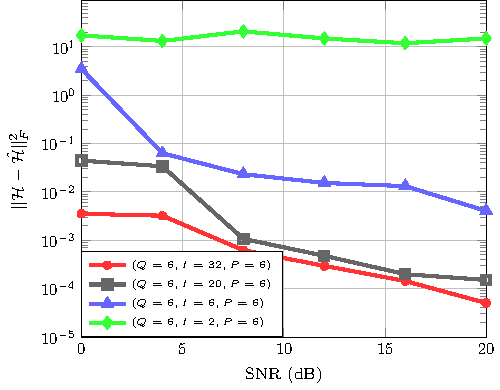
\includegraphics[width=0.5\textwidth]{fig/snr_nmse}
  \caption{Channel estimation using sparse PARAFAC model. }
  \label{fig:tx_beams}
\end{figure}

\begin{figure}[!thb]
  \centering
  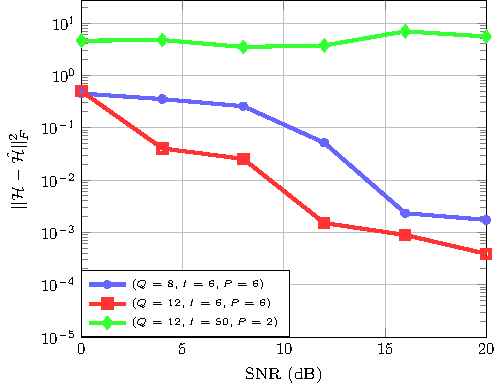
\includegraphics[width=0.5\textwidth]{fig/snr_nmse_rx}
  \caption{Channel estimation using sparse PARAFAC model. }
  \label{fig:tx_beams}
\end{figure}

\section{Conclusion}
The conclusion goes here.

\section*{Acknowledgment}

\bibliographystyle{IEEEtran}
\bibliography{latex-aux/reference}

\end{document}



%%% Local Variables:
%%% mode: latex
%%% TeX-master: t
%%% End:
